Simón camina en el desierto 2 kilómetros hacia el sur y luego un cierto número de kilómetros hacia el este.
Termina a 5 kilómetros de su posición inicial y se sienta a hacer el dibujo mostrado en la figura \ref{fig:proverb_pitagoras_01}:
\begin{figure}[H]
    \centering
    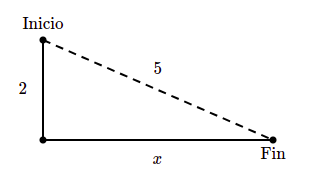
\includegraphics[width=0.35\linewidth]{../images/proverb_pitagoras_01.png}
    \caption{Dibujo elaborado por Simón antes de morir.}
    \label{fig:proverb_pitagoras_01}
\end{figure}

\textbf{¿Cuántos kilómetros caminó Simón hacia el este?}\\
\textit{Redondea tu respuesta a la décima de km más cercano.}

\begin{solutionbox}{8cm}
    Podemos usar el teorema de Pitágoras para obtener $x$.
    La ecuación del teorema de Pitágoras es:
    \[c^2=a^2+b^2\]
    donde $a$ y $b$ son las longitudes de los dos catetos del triángulo y $c$ es la longitud de la hipotenusa.
    En este caso, $a=2$, $b=x$ y $c=5$.
    \begin{align*}
        5^2       & =2^2+x^2  \\
        25        & = 4 + x^2 \\
        25-4      & =x^2      \\
        21        & =x^2      \\
        \sqrt{21} & =x        \\
        4.6       & \sim x    \\
    \end{align*}
    Simón caminó aproximadamente 4.6 kilómetros hacia el este.
\end{solutionbox}